\scanpage{151}
UNIVERSITE\\
DES SCIENCES ET TECHNIQUES\\
DU LANGUEDOC\\
------------

MONTPELLIER, le 17 Septembre 1980

Service de la Scolarité\\
MA/GJ\\
Diffusion : Liste A\\
N° : 4660

\uline{AVIS DE SOUTENANCE D'UNE THESE DE DOCTORAT DE 3ème CYCLE}

\uline{ENDOCRINOLOGIE}

\uline{Nom et prénom du candidat} : VIC Patrice

\uline{Titre de la thèse} : MODIFICATIONS ULTRASTRUCTURALES PRECOCES DE LA CHROMATINE INDUITES \uline{PAR LES OESTROGENES} DANS LES CELLULES EPITHELIALES DE L'UTERUS ET DES TUMEURS MAMMAIRES.

\uline{Date, heure et lieu de soutenance} : 6 OCTOBRE 1980 à 10 Heures\\
Salle de cours n° 9 - USTL

\uline{Nom du Directeur de thèse} : M. ROCHEFORT H.

\uline{Désignation du laboratoire où la thèse est préparée} : INSERMU 148 - Laboratoire d'endocrinologie moléculaire et cellulaire.

\uline{Résumé de la thèse} :

L'oestradiol transforme \uline{in vitro} et \uline{in vivo} en 60 min la chromatine condensée en chromatine dispersée. Ces modifications sont observées dans l'endomètre d'agnelle et de ratte impubères et dans les tumeurs mammaires hormono-dépendantes induites par le 7,12 Dimethylbenzanthracène, mais pas dans les tumeurs mammaires C3H hormonoindépendantes de souris. La DHT à dose pharmacologique a le même effet que l'oestradiol, alors que des hormones n'ayant pas d'affinité pour les récepteurs oestrogènes sont sans effet ; les antioestrogènes, comme le tamoxifène, provoquent à l'opposé une hypercondensation de la chromatine. Dans l'endomètre d'agnelle, cette décondensation de la chromatine serait une conséquence très rapidede la stimulation de la transcription. Ces résultats suggèrent sur le plan fondamental\unsure{:}que cette décondensation de la chromatine globale et précoce, serait due à une activité de nombreux gènes. Sur un plan pratique, ces observations pourraient constituer un test morphologique de prédiction de l'hormonodépendance dans les cancers du sein humain qui pourrait compléter le dosage des récepteurs hormonaux.

\uline{Durée approximative des recherches ayant abouti à la thèse} : 3 ans

\uline{Composition du jury proposé} :\\
MM. ASSENMACHER I.\\
SENTEIN P.\\
ROCHEFORT H.\\
Mme VIGNON F.

Pour le Secrétaire Général\\
L'Attachée d'Administration Universitaire

\figure{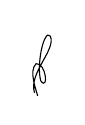
\begin{tikzpicture}[x=1cm,y=1cm]
\draw (0,0) .. controls (-.08,.25) and (.28,.55) .. (.20,.72) .. controls (.12,.82) and (.02,.35) .. (.08,.15) .. controls (.18,.02) and (.15,.38) .. (.02,.37) .. controls (-.08,.28) and (.03,.01) .. (.04,-.04);
\end{tikzpicture}}
\uline{\unsure{Gentil}}\\
\uline{A. GENTIL}

\margin{151}
